\section*{September 7, 2026: Natchez C excluded pending a site boundary}
\textit{Agent-drafted record; density exclusion approved by Jacob.}

The land review establishes that Natchez C's 16,031-square-foot denominator
covers only a fragment of its construction site. The eight residential buildings
cross the retained parcel and the excluded rail-corridor parcel. The retained
strip covers approximately 10--25 percent of each residential footprint; the
excluded corridor contains most of each building. Including the whole corridor
would also be incorrect because it extends well beyond the development.

Clipping the two parcels to the planned-development polygon gives approximately
86,560 square feet, but still omits part of the southern residence and about half
of the community center. Those structures extend onto the parcel assigned to B.
This alternative therefore does not establish a complete, nonoverlapping site for
C. The overlap measurements concern building footprints, not occupied floor area.

Jacob approved excluding C from density pending a reliable reviewed site boundary.
The existing density-exclusion ledger now contains seven records. The 39-unit
construction observation, its separate identity, and its accepted 2020 year are
preserved. A and B remain separate and unchanged. C already lies outside the
current main 500-foot sample, so adding this exclusion does not change that sample.
Wider samples must apply the exclusion when the reconstructed data are adopted.

\small
\textit{Reproduction and limits.} The release audit's two Natchez scripts produce
\path{natchez_building_land_coverage.csv} and \path{natchez_parcel_coverage.pdf}
through Make. The coverage file has nine unique footprint IDs: eight residences
and the community center. The new full 2022 footprint query returns 170 features
in its declared bounding box; the older scoped archive contained only four of
C's residences. Source files, including the adopted PD 1345 compilation, have
concrete acquisition rules and recorded checksums. The 2025 zoning polygon is
used only to test the proposed clipping method, not as a verified 2020 boundary.
The ordinary final exporter already reads the density-exclusion ledger and
retains rows while disabling both density measures. The upstream reconstruction
remains incomplete, and the frozen paper data are unchanged. The logbook build
holds the same three unrelated existing audit outputs fixed and reuses the
checksum-verified Grove and Northmarq source snapshots after an unrelated
Northmarq refresh failed DNS resolution.
\normalsize

\clearpage
\begin{center}
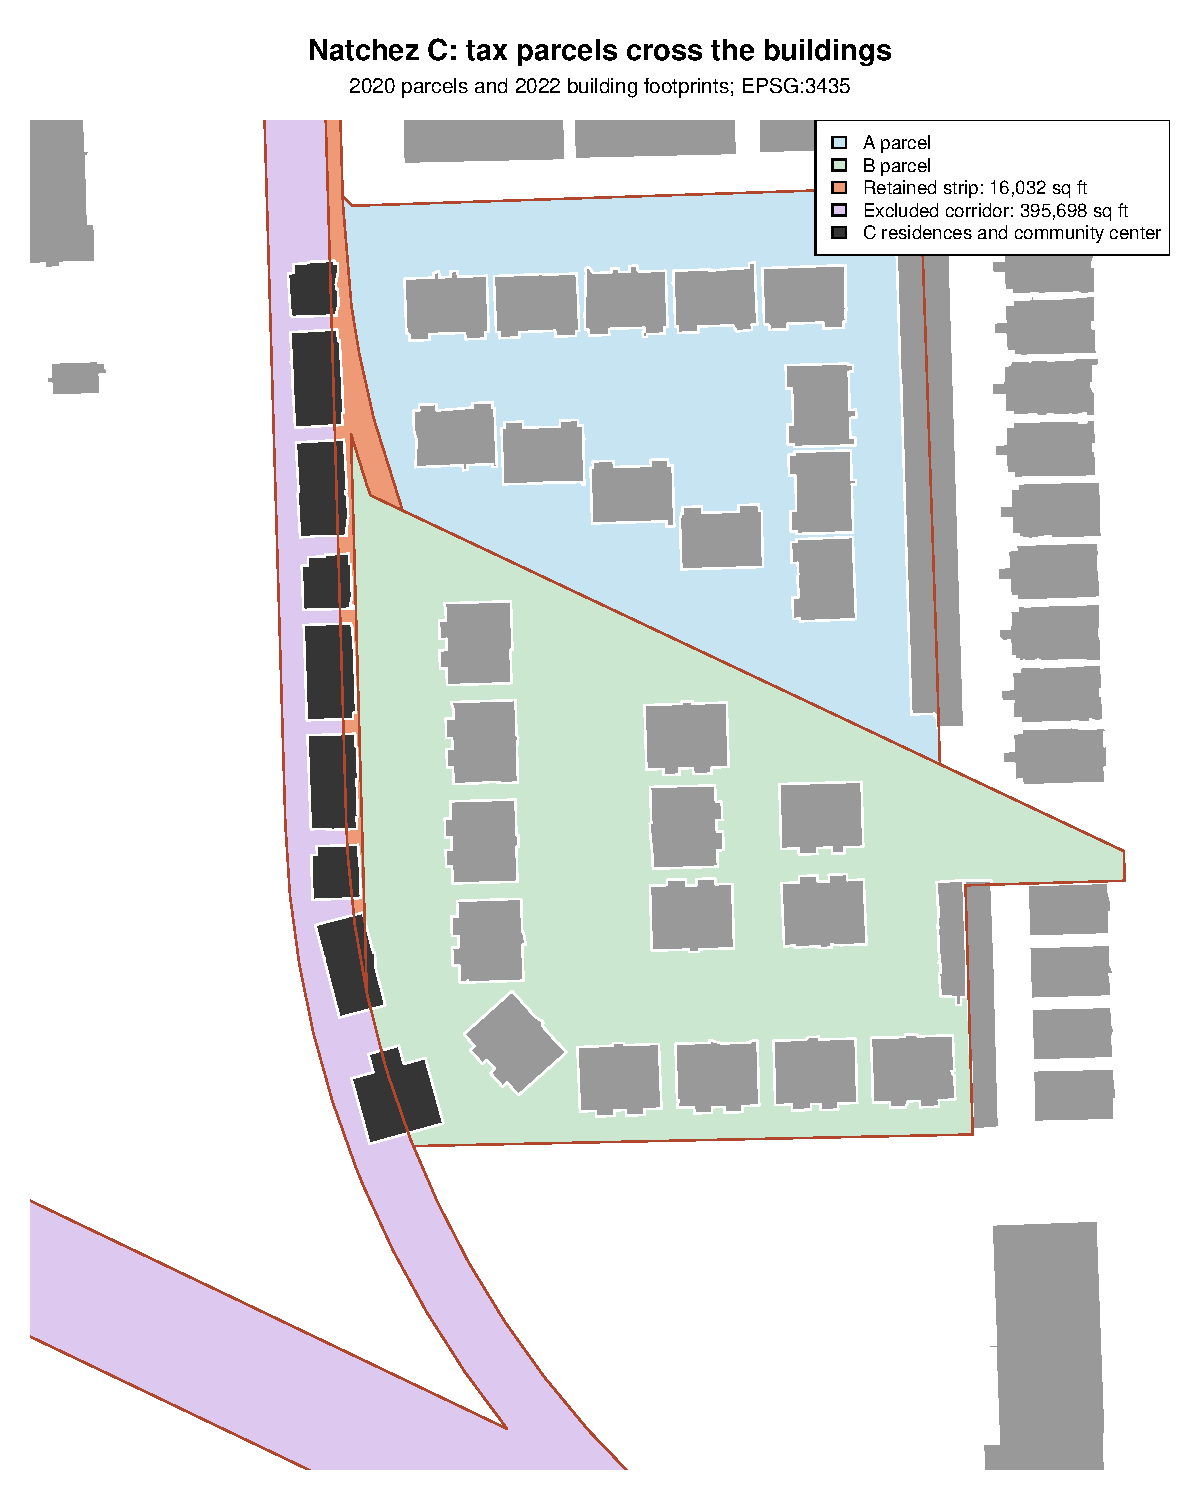
\includegraphics[height=0.88\textheight]{../tasks/audits/construction_review_history/records/natchez_parcel_coverage.pdf}
\end{center}
